% Chapter X

\chapter{Estensione del caso di studio alle linee ferroviarie} 

La rete ferroviaria dell'Abruzzo comprende linee che si sviluppano per un totale di circa 834 km di lunghezza, suddivise in nove tratte:

\begin{enumerate}
	\item Bologna - Bari
	\item Roma - Pescara
	\item Ortona - Crocetta
	\item Marina di San Vito - Castel di Sangro
	\item Teramo - Giulianova
	\item Avezzano - Roccasecca
	\item Sulmona - Carpinone
	\item Rieti - L'Aquila - Sulmona
	\item Archi stazione - Atessa
\end{enumerate}

Le tratte sono rappresentate in figura \ref{abruzzo_tratte}.

\begin{figure}[h]
	\centering
	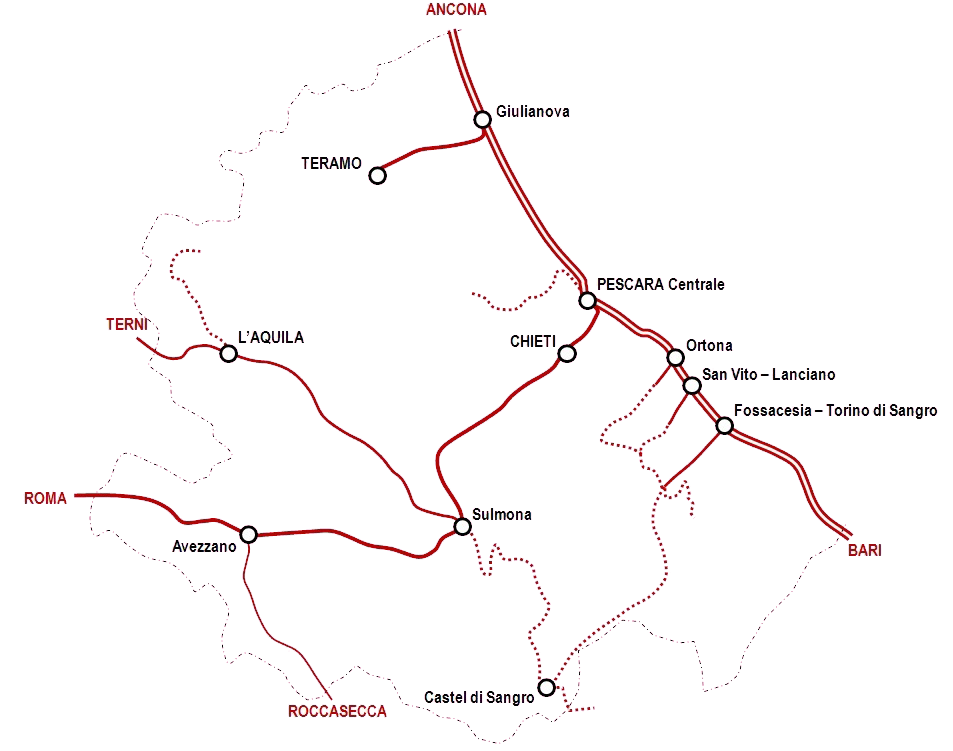
\includegraphics[width=0.6\textwidth]{images/Mappa_ferrovie_abruzzesi}
	\caption{Tratte ferroviarie abruzzesi.}
	\label{abruzzo_tratte}
\end{figure}

I dati relativi alle tratte sono stati importati nel progetto attraverso lo shapefile "railway\_routes". 
